\documentclass[11pt,spanish]{article}
\usepackage[utf8]{inputenc}
\usepackage{babel}
\usepackage{fullpage}
\usepackage{listings}
\usepackage{mathpazo}
\usepackage{enumitem}
\usepackage{courier}
\usepackage{xcolor}
\usepackage{textcomp}
\usepackage{amsmath}
\usepackage{amssymb}
\usepackage{tikz}
\usepackage{fancyhdr}
\usepackage{graphics}
\usepackage{array}
\usepackage{wasysym}
\usetikzlibrary{arrows}

\newcommand{\titulo}{Certamen para alumnos pendientes, viernes 11/11/11}
\newcommand{\cc}[1]{\hfil\texttt{#1}\hfil}
\newcommand{\pond}[1]{[{\small\textbf{#1\%}}]}

\pagestyle{fancy}
\lhead{%
  {\Large\bfseries Programación---\titulo} \\
  Nombre: \nombre\hfill
  Rol:    \rol
  \vspace{2ex}
}
\chead{}\rhead{}\lfoot{}\cfoot{}\rfoot{}
\renewcommand{\headrulewidth}{0pt}
\addtolength{\headheight}{7ex}
\headsep=4ex


\newcommand{\onelinerule}{\rule[2.3ex]{0pt}{0pt}}
\newcommand{\twolinerule}{\rule[6.2ex]{0pt}{0pt}}
\newcommand{\respuesta}{\framebox[\textwidth]{\twolinerule}}
\newcommand{\nombre}{%
  \begin{tikzpicture}[xscale=.4,yscale=.7]
    \draw (0, 0) rectangle (22, 1);
  \end{tikzpicture}%
}
%\newcommand{\rol}   {\framebox[0.3\textwidth]{\onelinerule}}
\newcommand{\rol}{%
  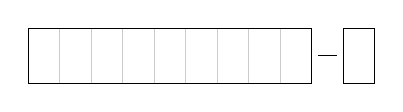
\begin{tikzpicture}[xscale=.4,yscale=.7]
    \draw[gray!40] ( 0, 0) grid      ( 9, 1);
    \draw          ( 0, 0) rectangle ( 9, 1);
    \draw          (10, 0) rectangle (11, 1);
    \draw (9 + .2, .5) -- (10 - .2, .5);
  \end{tikzpicture}%
}
\newcommand{\li}{\lstinline}
\providecommand{\pond}[1]{[{\small\textbf{#1\%}}]}

\lstdefinelanguage{py}{%
  classoffset=0,%
    morekeywords={%
      False,class,finally,is,return,None,continue,for,lambda,try,%
      True,def,from,nonlocal,while,and,del,global,not,with,print,%
      as,elif,if,or,yield,assert,else,import,pass,break,except,in,raise},%
    keywordstyle=\color{black!80}\bfseries,%
  classoffset=1,
    morekeywords={int,float,str,abs,len,raw_input,exit,range,min,max,%
      set,dict,tuple,list,bool,complex,round,sum,all,any,zip,map,filter,%
      sorted,reversed,dir,file,frozenset,open,%
      array,zeros,ones,arange,linspace,eye,diag,dot},
    keywordstyle=\color{black!50}\bfseries,%
  classoffset=0,%
  sensitive=true,%
  morecomment=[l]\#,%
  morestring=[b]',%
  morestring=[b]",%
  stringstyle=\em,%
}

\lstdefinelanguage{testcase}{%
  moredelim=[is][\bfseries]{`}{`},%
  backgroundcolor=\color{gray!20},%
}

\lstdefinelanguage{file}{%
  frame=single,%
}

\lstset{language=py}
\lstset{basicstyle=\ttfamily}
\lstset{columns=fixed}
\lstset{upquote=true}
\lstset{showstringspaces=false}
\lstset{rangeprefix=\#\ }
\lstset{includerangemarker=false}

\newlist{certamen}{enumerate}{1}
\setlist[certamen]{%
  label=\arabic*.,
  font=\LARGE\bfseries,%
  labelindent=-.5in,%
  leftmargin=0pt,%
  labelsep=1em%
}



\begin{document}

  \begin{enumerate}[font=\Large\bfseries]

    % Entender programas
    %\item%[1a.]
    %  \pond{25}
    %  Indique qué es lo que imprimen los siguientes programas.

    %  \foreach \x in {1,2,...,8} {
    %    \noindent
    %    \begin{minipage}[b]{19.8em}
    %      \lstinputlisting{p\x.py}
    %      \framebox[18em]{\rule[6ex]{0pt}{0pt}}
    %      \vspace{0.7em}
    %    \end{minipage}
    %  }

    \newpage
    \item
      \pond{33\(\frac{1}{3}\)\!}
      En un campo de batalla
      hay objetivos que se desea destruir (\frownie).
      Todos los objetivos están representados
      como tuplas \verb+(x, y)+
      indicando su posición en el campo.

      \begin{minipage}{0.65\textwidth}
        A su vez,
        en el campo hay varias posiciones amigas (\smiley)
        que se desea proteger.
        Las posiciones amigas también están representadas
        como tuplas \verb+(x, y)+.
        \\[1ex]
        Durante la próxima misión,
        se lanzarán varias bombas sobre el campo de batalla.
        Cada bomba está representada
        como una tupla \verb+(x, y, r)+,
        donde \verb+x+ e \verb+y+ indican el punto de impacto
        y \verb+r+ es el radio de acción de la bomba.
        Al caer en el punto de impacto,
        una bomba destruye todo lo que está
        a una distancia menor o igual que \verb+r+.
      \end{minipage}
      \hfill
      \begin{minipage}{.25\textwidth}
        \hfill
        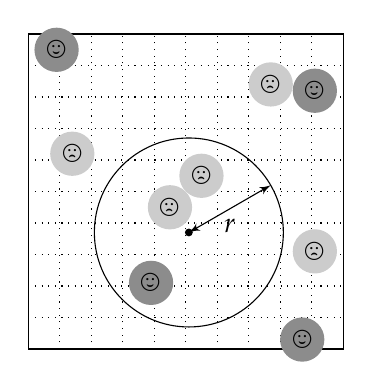
\begin{tikzpicture}[scale=.4, auto]
          \tikzstyle{target}=[inner sep=2pt, circle, fill=gray!40]
          \tikzstyle{friend}=[inner sep=2pt, circle, fill=gray!90]
          \draw[dotted] (0, 0) grid (10, 10);
          \draw (0, 0) rectangle (10, 10);
          \node[friend] (f0) at (3.9, 2.1) {\smiley};
          \node[friend] (f1) at (8.7, 0.3) {\smiley};
          \node[friend] (f2) at (9.1, 8.2) {\smiley};
          \node[friend] (f3) at (0.9, 9.5) {\smiley};
          \node[target] (t0) at (5.5, 5.5) {\frownie};
          \node[target] (t1) at (4.5, 4.5) {\frownie};
          \node[target] (t2) at (1.4, 6.2) {\frownie};
          \node[target] (t3) at (7.7, 8.4) {\frownie};
          \node[target] (t4) at (9.1, 3.1) {\frownie};
          \draw (5.1, 3.7) circle (3cm);
          \draw[latex'-latex'] (5.1, 3.7) --
              node [midway, below] {\(r\)}
              +(30:3cm);
          \node[inner sep=1pt, fill, circle] at (5.1, 3.7) {};
        \end{tikzpicture}
      \end{minipage}

      \begin{enumerate}
        \item Escriba la función \verb+contar_impactos(bomba, objetivos, amigos)+.
          La función debe retornar dos valores:
          la cantidad de objetivos destruidos por la bomba
          y la cantidad de posiciones amigas destruidas por la bomba.
          Los parámetros \verb+objetivos+ y \verb+amigos+
          son listas de objetivos y posiciones amigas, respectivamente.

        \item
          Una bomba es útil si destruye por lo menos un objetivo
          y no destruye ninguna posición amiga.

          Escriba la función \verb+bombas_utiles(bombas, objetivos, amigos)+,
          que recibe como primer parámetro una lista de bombas,
          y retorna una nueva lista que contiene sólo las bombas que son útiles.
      \end{enumerate}

    \newpage
    \item
      \pond{33\(\frac{1}{3}\)\!}
      En un campeonato de fútbol de eliminación directa, los equipos se enfrentan de a pares.
      Para cada uno de los enfrentamientos se juegan dos partidos:
      uno \emph{de ida} y uno \emph{de vuelta}.
      El partido de ida se juega en el estadio del primer equipo,
      y el partido de vuelta en el del segundo.
      En cada partido, el equipo que juega en su propio estadio se llama \emph{local},
      y el otro es la \emph{visita}.

      Los resultados de los partidos están registrados en el archivo de texto \texttt{ronda1.txt},
      en el que cada línea tiene cuatro datos separados por el símbolo ``\verb+:+'':
      los dos equipos, el resultado de la ida y el resultado de la vuelta.

      Al final de los dos partidos,
      se suman los goles anotados por ambos equipos.
      El equipo que anotó más goles en total clasifica para la ronda siguiente,
      y el otro queda eliminado.

      Si ambos equipos anotaron la misma cantidad total de goles,
      el equipo que clasifica es el que anotó más goles jugando de visita.
      Si los equipos empatan tanto en goles totales como en goles de visita,
      entonces clasifica el que jugó de visita el partido de vuelta.

      Los equipos que clasifican a la ronda siguiente se enfrentan nuevamente de a pares.
      Los nuevos enfrentamientos se forman tomando los equipos clasificados de dos en dos,
      en el mismo orden en que aparecen en el archivo.

      Escriba un programa que,
      a partir de los resultados registrados en el archivo \texttt{ronda1.txt},
      determine cuáles equipos clasificaron,
      y genere un nuevo archivo llamado \texttt{ronda2.txt}
      con los partidos que se jugarán en la ronda siguiente.
      Siga el formato del ejemplo.

      El archivo \texttt{ronda1.txt} tiene una cantidad par de líneas,
      pero que usted no conoce de antemano.

      \begin{minipage}[t]{.28\textwidth}
        Archivo \texttt{ronda1.txt}:
        \lstinputlisting[frame=single]{ronda1.txt}
      \end{minipage}
      \hspace{3em}
      \begin{minipage}[t]{.28\textwidth}
        Archivo \texttt{ronda2.txt}:
        \lstinputlisting[frame=single]{ronda2.txt}
      \end{minipage}

    \newpage
    \item
      \pond{33\(\frac{1}{3}\)\!}
      La red social Cakeboof almacena la información de sus usuarios en una lista,
      cuyos valores son tuplas con el nombre, la ciudad y la fecha de nacimiento del usuario.
      La fecha de nacimiento es una tupla \texttt{(año, mes, día)}.
      El código de cada usuario está dado por su posición en la lista:
      \lstinputlisting[linerange=USUARIOS-FIN\ USUARIOS]{cakeboof.py}

      Para guardar la información sobre cuáles de sus usuarios son amigos entre sí,
      Cakeboof utiliza el arreglo bidimensional \li!amistades!.
      Si los usuarios \li+A+ y \li+B+ son amigos,
      entonces \li!amistades[A, B]! tiene el valor uno,
      y si no lo son, tiene el valor cero:
      \lstinputlisting[linerange=AMISTADES-FIN\ AMISTADES]{cakeboof.py}

      \begin{enumerate}
        \item Escriba la función \li!obtener_amigos(i)!,
          que retorne el conjunto de los amigos de \li!i!.
        \item Escriba la función \li!tienen_amigos_en_comun(i, j)!,
          que indique si \li!i! y \li!j! tienen amigos en común.
        \item Escriba la función \li!recomendar_amigos(i)!,
          que retorne el conjunto de los usuarios
          que son amigos de un amigo de \li!i!,
          pero que no son amigos de \li!i!.
      \end{enumerate}
      \lstinputlisting[language=py, linerange=CASO-FIN\ CASO]{cakeboof.py}

  \end{enumerate}
\end{document}

